%%%%%%%%%%%%
%
% $Autor: Wings $
% $Datum: 2019-03-05 08:03:15Z $
% $Pfad: Automatisierung/Skript/Produktspezifikation/Powerpoint/AMF.tex $
% $Version: 4250 $
%
%%%%%%%%%%%%


%zusammenführen
\subsection{CIFAR-10 and CIFAR-100}
\index{Dataset!CIFAR-10}\index{Dataset!CIFAR-100}




\subsubsection{Data Set \ac{cifar}-10}\label{sec:dataset}

The data sets \ac{cifar}-10 and \ac{cifar}-100 \index{Dataset!CIFAR-10}\index{Dataset!CIFAR-100} were developed by Alex Krizhevsky and his team and therefore named after the \textbf{C}anadian \textbf{I}nstitute \textbf{f}or \textbf{A}dvanced \textbf{R}esearch\index{Canadian Institute for Advanced Research}.  



The data set \ac{cifar}-10 is a partial data set of the data set \emph{80 Million Tiny Images}. This part consists of 60,000 images, divided into 50,000 training images and 10,000 test images, which are divided into 10 classes and labelled accordingly. The existing classes represent aeroplanes, cars, birds, cats, deer, dogs, frogs, horses, ships and trucks. Thus, 6,000 images exist per class, with each image having a size of $32\times32$ pixels with three colour channels \cite{Krizhevsky:2009,Krizhevsky:2017}. An extract of the dataset can be seen in \cref{fig:cifar-example}.

\begin{figure}[htb]
	\centering
	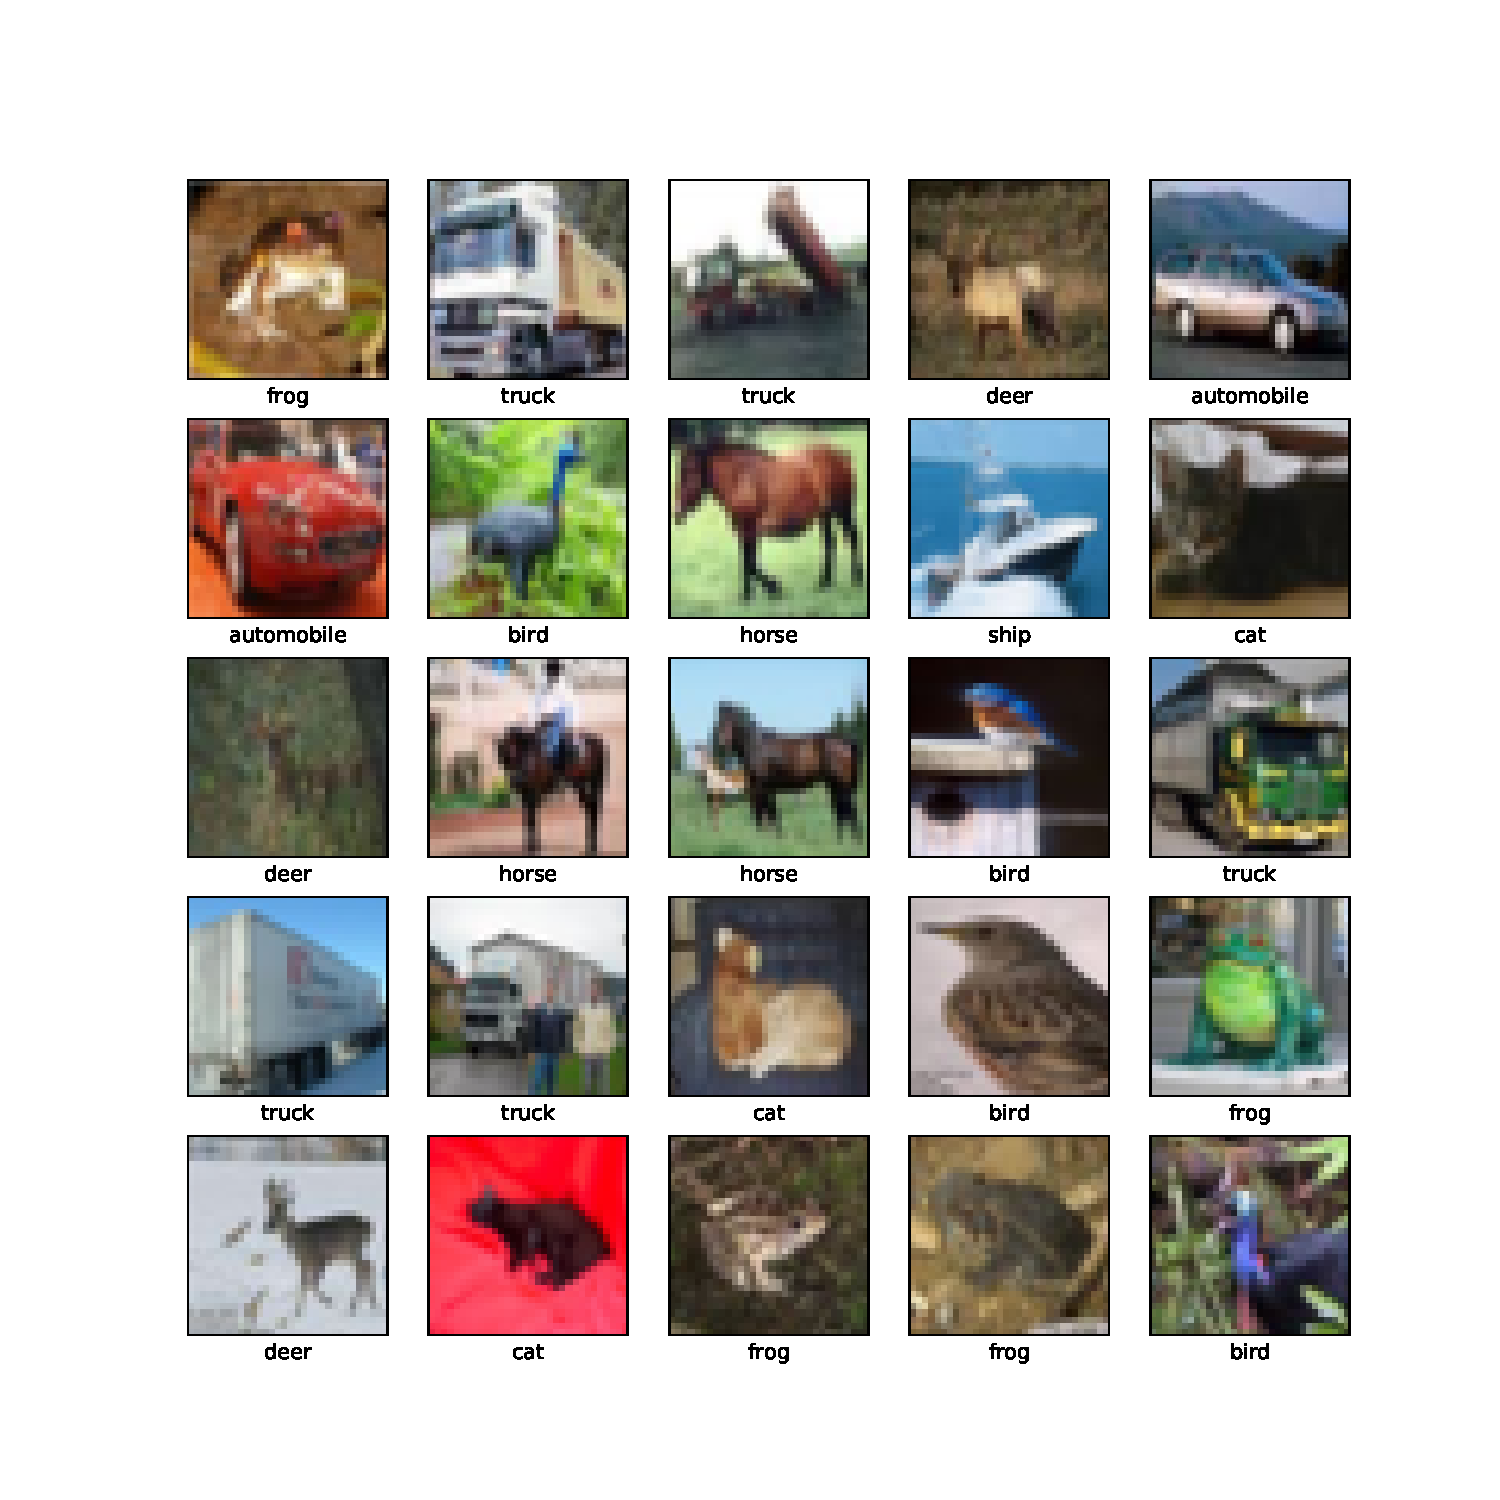
\includegraphics[trim = 25mm 145mm 25mm 15mm, clip, width=\textwidth]{CUDA/cifar-sample.pdf}
	\caption{Extract from ten illustrations of the data set \ac{cifar}-10}
	\label{fig:cifar-example}
\end{figure}

To import the dataset into the Python environment, the module \python{keras.datasets} is used here. This contains a direct interface to the dataset \ac{cifar}-10, which is downloaded to the local system by calling the function \PYTHON{load\_data()}. In the background, the dataset is downloaded as a packed file with the extension \mytt{.tar.gz} and stored in the folder \FILE{C:\textbackslash Users\textbackslash <username>\textbackslash .keras\textbackslash datasets}. After unpacking, the dataset is contained in several serialised objects, which are loaded into the Python environment via \PYTHON{pickle}. The training data, training labels, test data and test labels can then be accessed via corresponding lists (\cref{src:cifarimport}). In order to reduce the vanishing gradient problem during the later training, the RGB colour values stored in the data set with the value range from 9 to 255 are converted into values from 0 to 1. The listing~\ref{src:cifarimport} shows the loading and normalisation of the data.


\begin{code}
\begin{lstlisting}[language=MyPython, numbers=left,label={src:cifarimport}]
	(TRAIN_IMAGES, TRAIN_LABELS), (TEST_IMAGES, TEST_LABELS) =  datasets.cifar10.load_data()
	TRAIN_IMAGES = TRAIN_IMAGES / 255.0
	TEST_IMAGES  = TEST_IMAGES / 255.0
\end{lstlisting}
  \caption{Load and normalise the data set \ac{cifar}-10}
\end{code}


\subsubsection{Data Set \ac{cifar}-100}\label{sec:dataset}


The data set \ac{cifar}-100, on the other hand, also contains 60,000 images, but divided into 100 categories with 600 images each. In addition, there are 20 upper categories, to each of which five of the 100 categories are assigned; see table~\ref{TabCIF100}.

\begin{figure}
    \begin{tabular} {l l} 
        \hline
        Superclass &	Classes\\
        \hline
        aquatic mammals & 	beaver, dolphin, otter, seal, whale\\
        fish & 	aquarium fish, flatfish, ray, shark, trout\\
        flowers & 	orchids, poppies, roses, sunflowers, tulips\\
        food containers &	bottles, bowls, cans, cups, plates\\
        fruit and vegetables &	apples, mushrooms, oranges, pears, sweet peppers\\
        household electrical devices &	clock, computer keyboard, lamp, telephone, television\\
        household furniture &	bed, chair, couch, table, wardrobe\\
        insects &	bee, beetle, butterfly, caterpillar, cockroach\\
        large carnivores &	bear, leopard, lion, tiger, wolf\\
        large man-made outdoor things &	bridge, castle, house, road, skyscraper\\
        large natural outdoor scenes &	cloud, forest, mountain, plain, sea\\
        large omnivores and herbivores &	camel, cattle, chimpanzee, elephant, kangaroo\\
        medium-sized mammals &	fox, porcupine, possum, raccoon, skunk\\
        non-insect invertebrates &	crab, lobster, snail, spider, worm\\
        people &	baby, boy, girl, man, woman\\
        reptiles &	crocodile, dinosaur, lizard, snake, turtle\\
        small mammals &	hamster, mouse, rabbit, shrew, squirrel\\
        trees &	maple, oak, palm, pine, willow\\
        vehicles 1 &	bicycle, bus, motorcycle, pickup truck, train\\
        vehicles 2 &	lawn-mower, rocket, streetcar, tank, tractor\\
    \end{tabular}
    \caption{Supercategories and categories in \ac{cifar}-100 with the original designations}
    \label{TabCIF100}
    
\end{figure}


The dataset can also be downloaded and imported directly into TensorFlow via Keras \cite{kaggle.21.09.2020}:

\begin{code}
    
\begin{lstlisting}[language=MyPython, numbers=left,label={src:cifarimport}]
    import tensorflow as tf
    from tensorflow.keras import datasets
    
    (TRAIN_IMAGES100, TRAIN_LABELS100), (TEST_IMAGES100, TEST_LABELS100) = tf.keras.datasets.cifar100.load_data()
	TRAIN_IMAGES100 = TRAIN_IMAGES100 / 255.0
    TEST_IMAGES100  = TEST_IMAGES100 / 255.0
    
\end{lstlisting}
  \caption{Load and normalise the data set \ac{cifar}-100}
\end{code}

